\begin{frame}
    \frametitle{Higgs-BRs all-in-one}
    \setbeamercovered{transparent}
    \begin{columns}[c,onlytextwidth]
    \begin{column}{0.55\textwidth}
    \vfill
    \begin{enumerate}
        \item Build samples with all Higgs decay modes
            (Higgsstrahlung, $Z\to (e^+e^-, \mu^+\mu^-)$).
        \item<2-> Construct categories to separate the decay modes (\& background)
            as well as possible.
        \item<5-> Fit the Higgs branching ratios to the observed category counts.
    \end{enumerate}
    \end{column}
    \begin{column}{0.45\textwidth}
    \only<1>{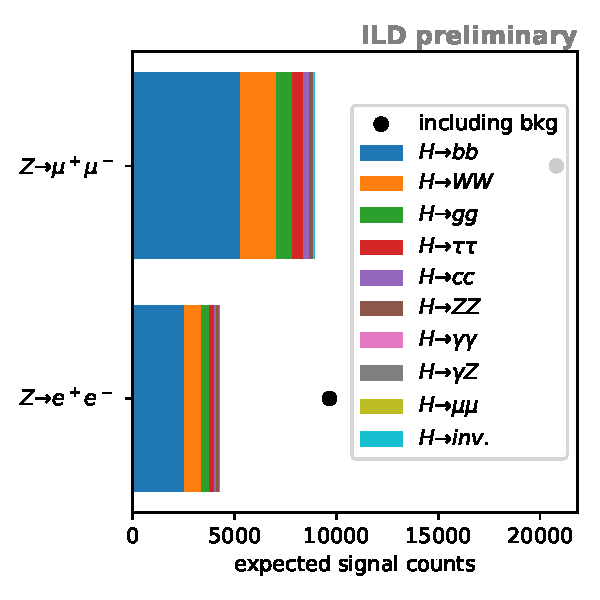
\includegraphics[height=0.75\textheight, width=0.95\textwidth, keepaspectratio]
        {intro_sample_counts}}
    \only<2>{\addtocounter{framenumber}{1} \put(0, 0){
        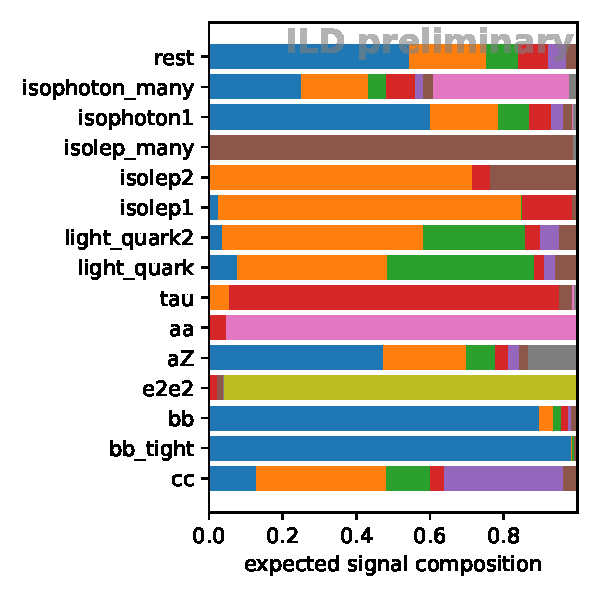
\includegraphics[height=0.75\textheight, width=0.95\textwidth, keepaspectratio]
        {intro_signal_composition_per_category}}}
    \only<3>{\addtocounter{framenumber}{1} \put(0, 0){
        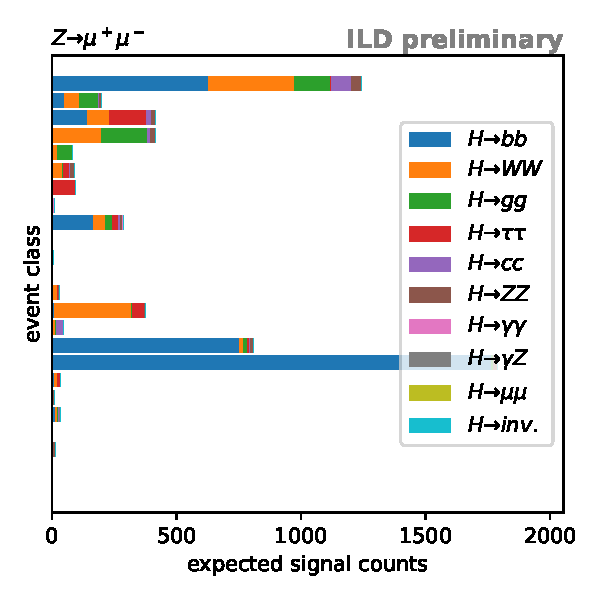
\includegraphics[height=0.75\textheight, width=0.95\textwidth, keepaspectratio]
        {intro_category_counts}}}
    \only<4>{\addtocounter{framenumber}{1} \put(0, 0){
        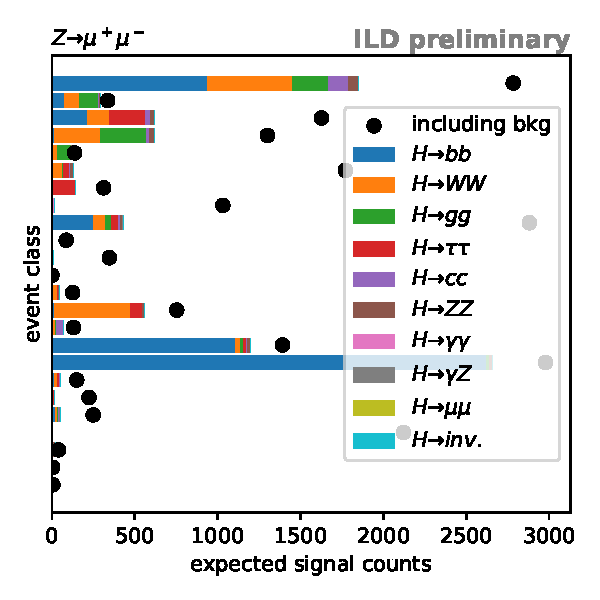
\includegraphics[height=0.75\textheight, width=0.95\textwidth, keepaspectratio]
        {intro_category_counts_w_bkg}}}
    \only<5>{\addtocounter{framenumber}{1} \put(0, 0){
        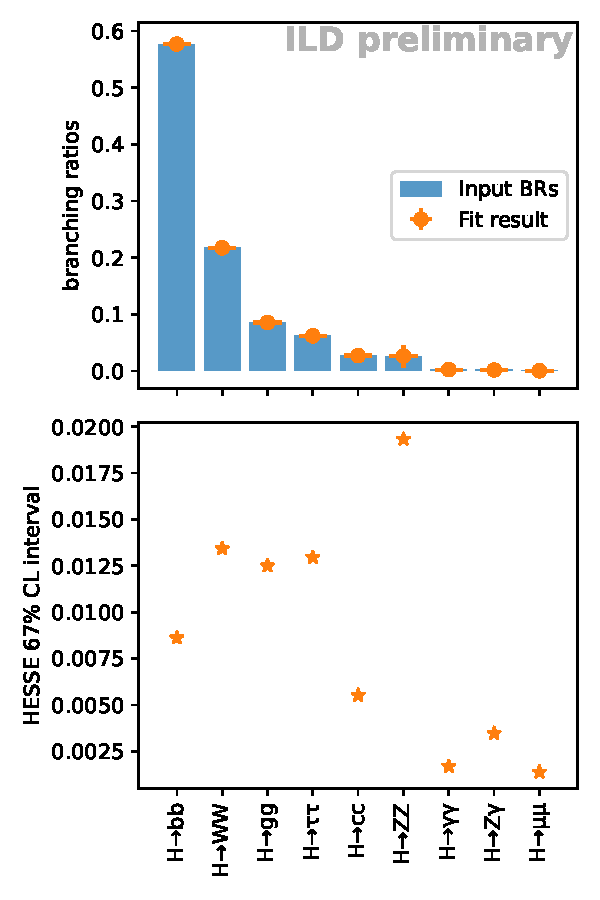
\includegraphics[height=0.75\textheight, keepaspectratio]
        {br_estimates}}}
    % \only<5>{\addtocounter{framenumber}{1}
    % \\
    % \textbf{Advantages}
    % \begin{itemize}
    %     \item A model independent extraction of all branching ratios (at once).
    %     \item Independent of any Higgs production cross section measurement.
    %     \item Gaussian errors $\rightarrow$ multinomial errors, as everything is in the same sample.
    %     \begin{itemize}
    %         \item Promising e.g. for $H \to b\bar{b}$.
    %             See {\color{llblue}\ref{many_likelihoods_optimizations}} in backup.
    %     \end{itemize}
    %   \end{itemize}}
    \end{column}
    \end{columns}
    % {\small
    % Similar to a $\tau$ branching ratio analysis at ALEPH:
    % \href{https://arxiv.org/abs/hep-ex/0506072}{\color{llblue} \texttt{arXiv:hep-ex/0506072}}.
    % }
    \end{frame}
